\documentclass[a4paper,titlepage,11pt]{ltjsarticle}
\usepackage{graphicx}
\usepackage{amssymb}
\usepackage{here}
\begin{document}
%%タイトル
  \title{システム開発入門\\第一回レポート}
  \author{2022531033 関川謙人\\d2531033@kitakyu-u.ac.jp}
  \maketitle

  %%%%%%一章%%%%%%%%
  \section{目的}

  %%%%%%%一節%%%%%%%%
  \subsection{}
  Labviewにおいて論理演算、四則演算、フロー制御を
  実験方式で学習する意義。それは、実際に開発現場において
  回路を組み込む際に、適切なシミュレーションを行う
  必要があることだと考える。例えば回路を組む際、ショートが発生するような
  回路であった場合に、実際に回路を組んでしまった場合であれば
  もはや取り返しがつかないが、事前にlabviewで検証できる知識があれば、
  そういった事故を防げうる。
  %%%%%%%%%二節%%%%%%%%%
  \subsection{}
論理回路の練習問題の中から一つ、(4)、NANDで(1)~(3)の問題で実現した内容を表す問題に
ついて。前提条件として、NANDは以下の状況下で以下の反応を示す。

%%%%表
\begin{tabular}{|c|c|c|}\hline
  A & B & NAND \\ \hline
  T & T & F \\ \hline
  F & T & T \\ \hline
  T & F & T \\ \hline
  F & F & T \\ \hline
\end{tabular}\label{nandtable}\ref{nandtable}
%%%%表ここまで

(4)-(1)について確認する。
この回路では、(1)で再現した内容であるボタンを両方ONにしたときにのみライトがつくといった
回路であるが、(1)においてはANDを用いてこの回路を再現したため、NANDでANDを表現する
問題と読み替えることができる。このとき、二つのボタンをそれぞれボタンA,ボタンBとすると、
AND=$A\cap B$と表せ、また
NAND=$(\overline{A\cap B} )$
である。即ちNANDを否定する回路を作る必要がある。
このとき

$A\cap B= \overline{\overline{A\cap B}\cap \overline{A\cap B}}$ \label{andnand}(\ref{andnand})

となるように回路を組む必要がある。
(4)-(2)において、この回路は数学的には、このように表せる

$\overline{A\cap B}= \overline{\overline{A}\cap\overline{B}}$。

(4)-(3)においては、(3)で再現した内容を数学的に表すと、

$\overline{A\cap B} \cap A\cup B$

と表せるが、この時orを表す$A\cup B$をNANDを用いて表す必要がある。
このとき、orは数学的に、

$A\cup B = \overline{\overline{A}\cap \overline{B}}$

これらを組み合わせると、

$\overline{(A\cap B)} \cap (\overline{\overline{A}\cap \overline{B}})$

と数学的には表せる。
電気回路練習問題の中から、(1)の問題を抜粋して解説する。
E1,E2,R1,R2,R3の値を提示したときにI1,I2,I3を表示する問題であるが、

この時、E1とE2で以下の配列を作る。

$Y=\left(
  \begin{array}{r}
  E_{1} \\
  E_{2}
  \end{array}
\right)$

また、抵抗値を使って、以下の配列を作る。

$A=\left(
  \begin{array}{rr}
  R_{1}+R_{3} \ R_{3} \\
  R_{3} \ R_{2}+R_{3}
  \end{array}
\right)$

また、この時、Y=AXであり、Xの配列がI1,I2を表す配列となるが、
このとき方程式の形は、

$\left(
  \begin{array}{r}
  E_{1} \\
  E_{2}
  \end{array}
\right)
=
\left(
  \begin{array}{rr}
  R_{1}+R_{3} \ R_{3} \\
  R_{3} \ R_{2}+R_{3}
  \end{array}
\right)
\left(
  \begin{array}{r}
  I_{1} \\
  I_{2}
  \end{array}
\right)
$

また、X行列を詳細に表すと、

$X=\left(
  \begin{array}{r}
I_{1}=\frac{(R_{2}+R_{3}E_{1})-R_{3}E_{2}}
{R_{1}R_{2}+R_{2}R_{3}+R_{3}R_{1}} \\
I_{2}=\frac{(R_{1}+R_{3}E_{2})-R_{3}E_{1}}
{R_{1}R_{2}+R_{2}R_{3}+R_{3}R_{1}}
  \end{array}
\right)$

となる。

また、

$I_{3}=I_{1}+I_{2}$

である。

この場合、この回路は電圧と抵抗からなる配列の方程式を解き、
その時の電流の値を解とする。この時、AX=Yのうち
Xは電流、Yは電圧、Aは抵抗に対応しており、ベクトルの式を
用いて比較的効率的に計算できることを示している。また、
この式はオウムの法則に対応している。

判定反復問題においては、BMIを表示するツールを作成した。
このとき$体重/身長^2$でBMIが求められるので、この時求めたBMIの値を
$x$としたとき、

$x<18.5$のとき、「underweight」、

$18.5 \leqq x<25$のとき、「normal range」

$25 \leqq x <30$のとき、「pre-obese」

$30<x$のとき、「obese」と表示するプログラムとなる。

これを再現すればよい。

%%%%%%2章%%%%%%%%
\section{実験方法}
(4)-(1)のブロックダイヤグラムは以下の画像の通りである。
\begin{figure}[H]
  \begin{center}
    \includegraphics[width=100mm]{4-2b.pdf}
    \caption{(4)-(1)}
  \end{center}
\end{figure}

A,Bを各NANDに一つづつ接続、そのうえで各NANDの出力結果を一つのNANDに接続すれば、NANDを用いて
ANDを再現することができ、(1)をNANDを用いて表せる。

同様に、(4)-(2)について、

\begin{figure}[H]
  \begin{center}
    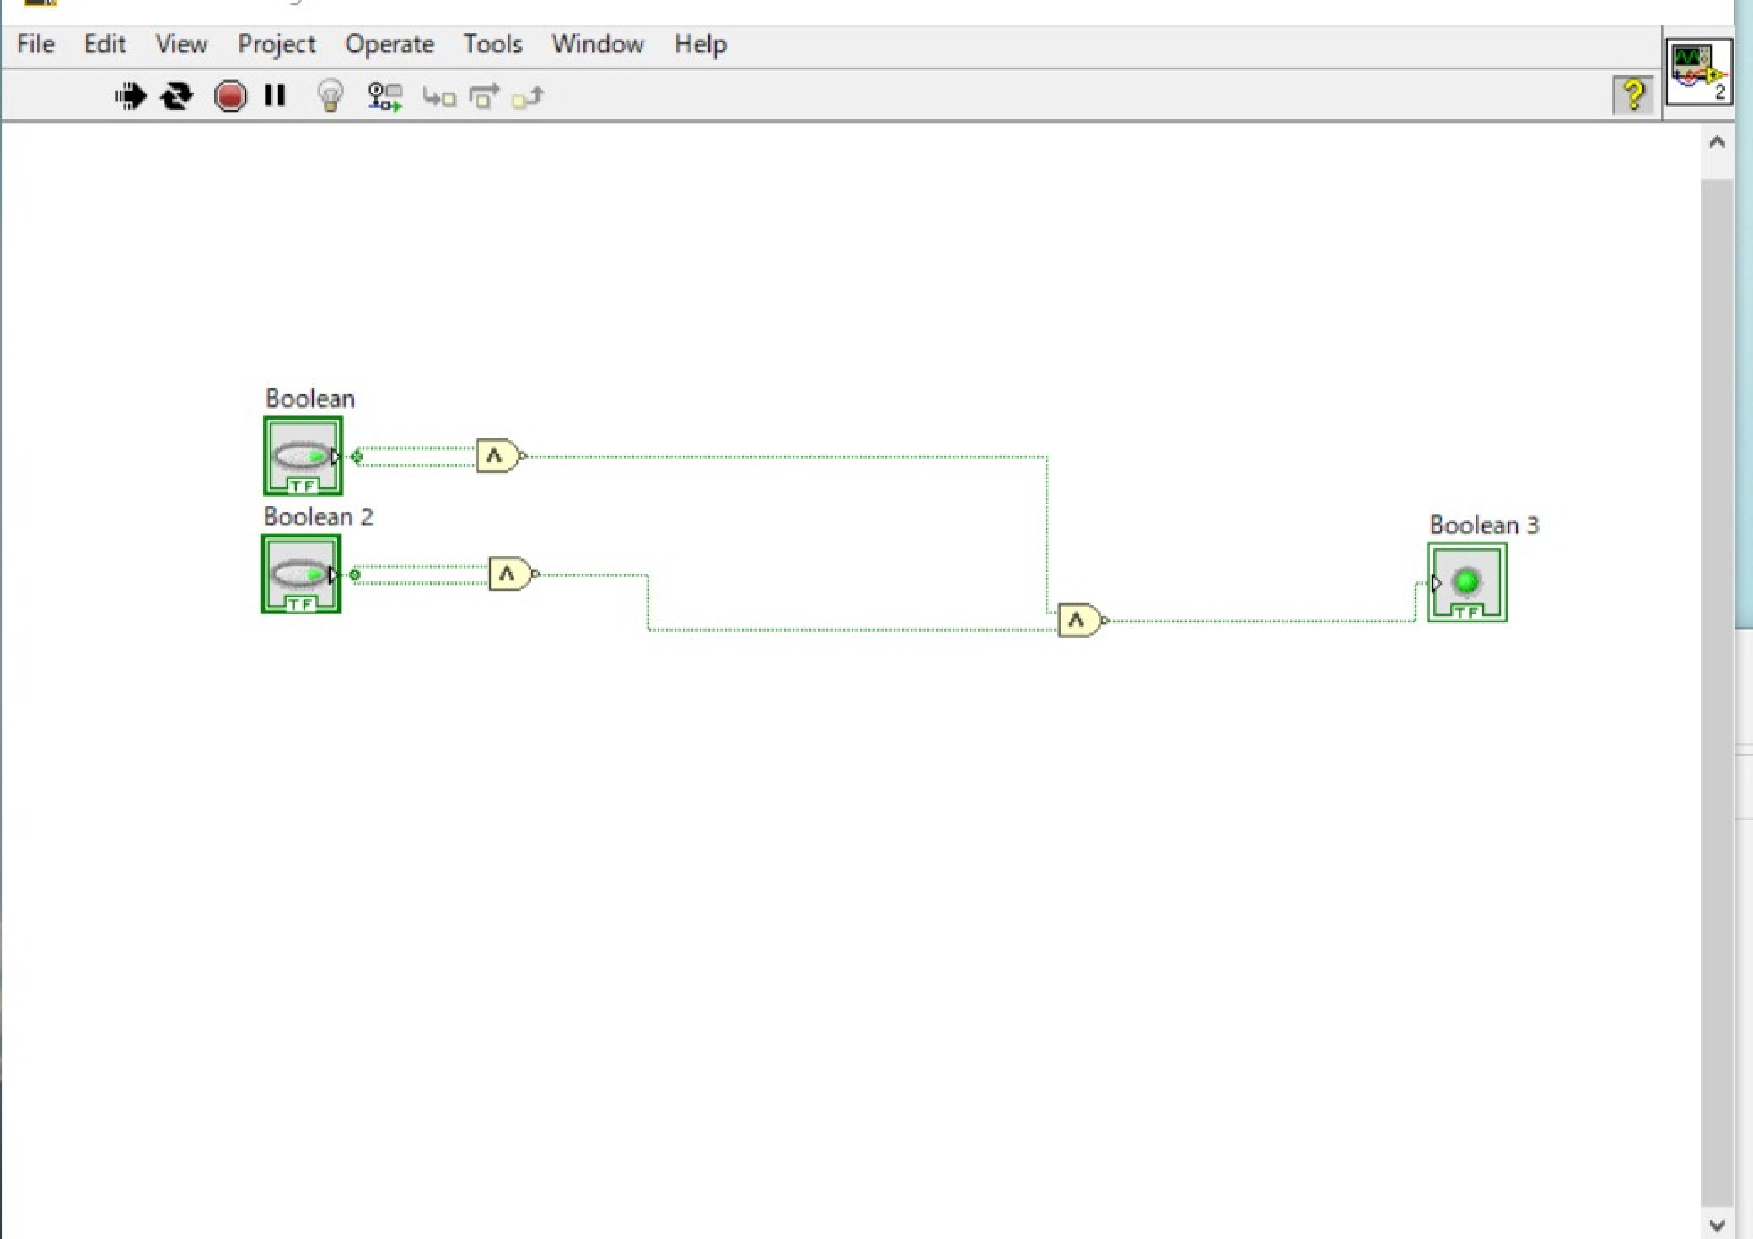
\includegraphics[width=100mm]{4-1b.pdf}
    \caption{(4)-(2)}
  \end{center}
\end{figure}

(4)-(2)において、先ほど作った(4)-(1)の問題の否定を
再現する必要があるが、この時表(\ref{nandtable})より、
NANDには同じ要素を提示されたとき、両方Falseだった場合は
Trueを、Trueだった場合はFalseを返す性質をもつ。この性質を利用して、各ボタンから
二つの導線をNANDにつなぎ、そのうえで(1)で再現したように、各NANDの返す要素を一つの
NANDにつなぐことで、(2)をNANDを用いて再現できる

同様に、(4)-(3)について、

\begin{figure}[H]
  \begin{center}
    \includegraphics[width=100mm]{4-3b.pdf}
    \caption{(4)-(3)}
  \end{center}
\end{figure}

二つの導線をNANDにつなぎ、またその出力結果をそれぞれNANDに接続して
orを表す。これを\alpha とする。またもう片方はそれぞれのNANDにそのまま接続する。これを\beta とする。またNANDで
andを再現する。これを\gamma とする。\alpha 、\beta の出力結果をそれぞれ\gamma に接続するとそれが(4)-(3)の回答となる。

電気回路練習問題において、(1)については、以下の画像の通り。

\begin{figure}[H]
  \begin{center}
    \includegraphics[width=100mm]{electronics1b.pdf}
    \caption{電気回路練習問題(1)}
  \end{center}
\end{figure}

線形代数学を扱う回路となっているが、E1とE2をBuild matrixコンテクストを使用して
縦のベクトルとして扱えるようにし、R1+R3,R3、また、R2,R3でそれぞれ横ベクトル
を構築したうえでそれらを縦二列に合わせ、正方形ベクトルを構成する。
そのうえでSolve Linear Equationsコンテクストを利用する。このコンテクストは
Y=AXの式にユーザーがYの行列とAの行列を代入し、その結果をもとにXを解として出力する
ものである。出力された解のうち一列目がI1,二列目がI2である。この結果の行列から数値を抽出するコンテクストであるGet Matrix Element
コンテクストを利用し、I1、I2をそれぞれ抽出してI1,I2として表示、またI3は
I1+I2であるので、I1,I2を足し算コンテクストに接続するだけである。
※\cite{sankoga}を模倣

判定処理問題の練習問題には、(3)に取り組んだ。

\begin{figure}[H]
  \begin{center}
    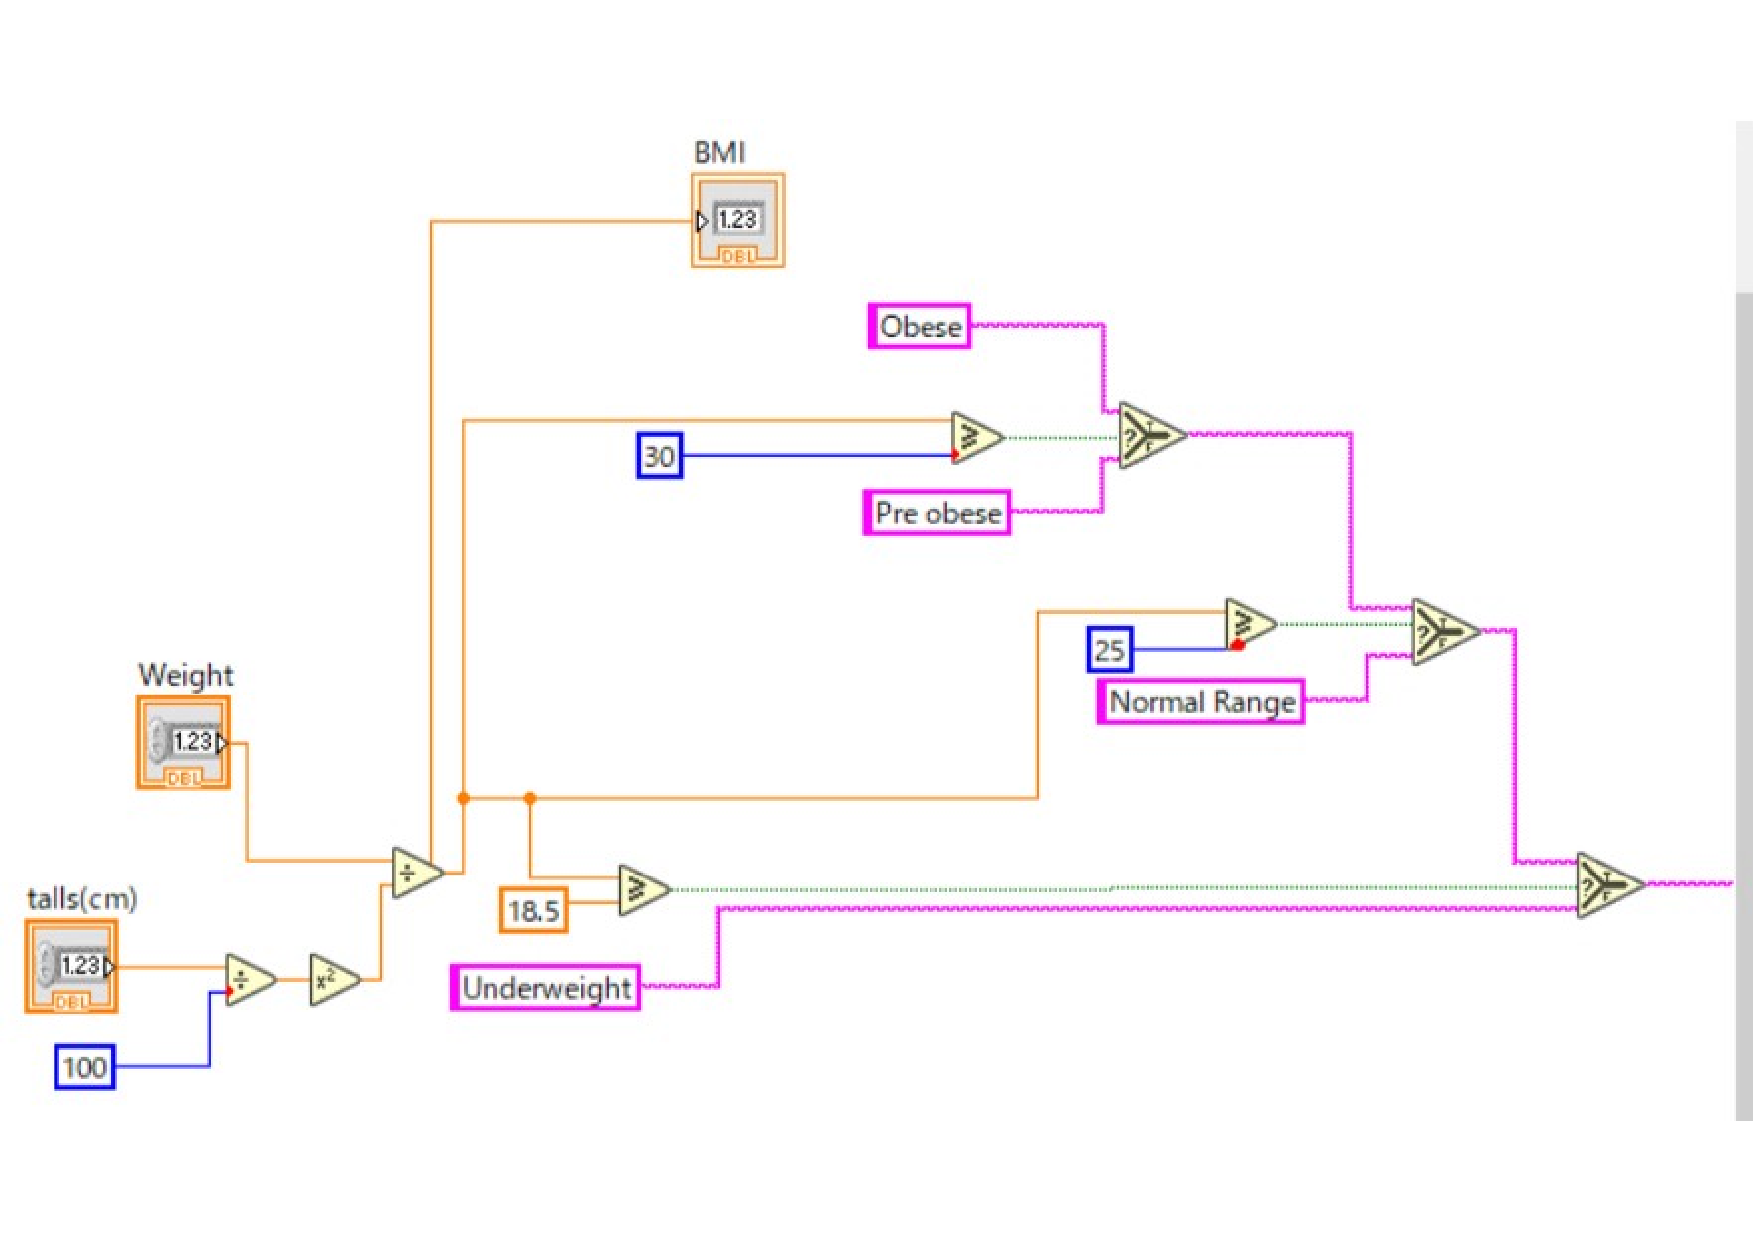
\includegraphics[width=100mm]{jadge3.pdf}
    \caption{判定処理練習問題(3)}
  \end{center}
\end{figure}

BMIの求め方は先ほど説明したが、今度は判定について説明する。
selectコンテクストの活用によって、case structureを使用することで
生じるプログラムの複雑化を防ぐことができた。selectの仕組みは、
真ん中に判定結果を入力し、Trueだった場合は、Trueにつながった挙動を、
Falseだった場合はFalseにつながった挙動をするようになっている。
このとき、さかのぼってNormal Rangeの条件を満たした場合、次の判定へ、
満たさなかった場合はUnderweightと表示するといった具合に判定を重ね、
肥満度を表示する仕組みにしている。また、BMIを求めやすいよう、
cmで入力させる仕組みにしている。

  %%%%%%三章%%%%%%%%
  \section{実験結果}
  (4)-(1)について、ボタンを両方オンにしたとき、ライトは点灯した。また、
  片方オフにするなどの動作を試したが、ライトは点灯しなかった。

  \begin{figure}[H]
    \begin{center}
      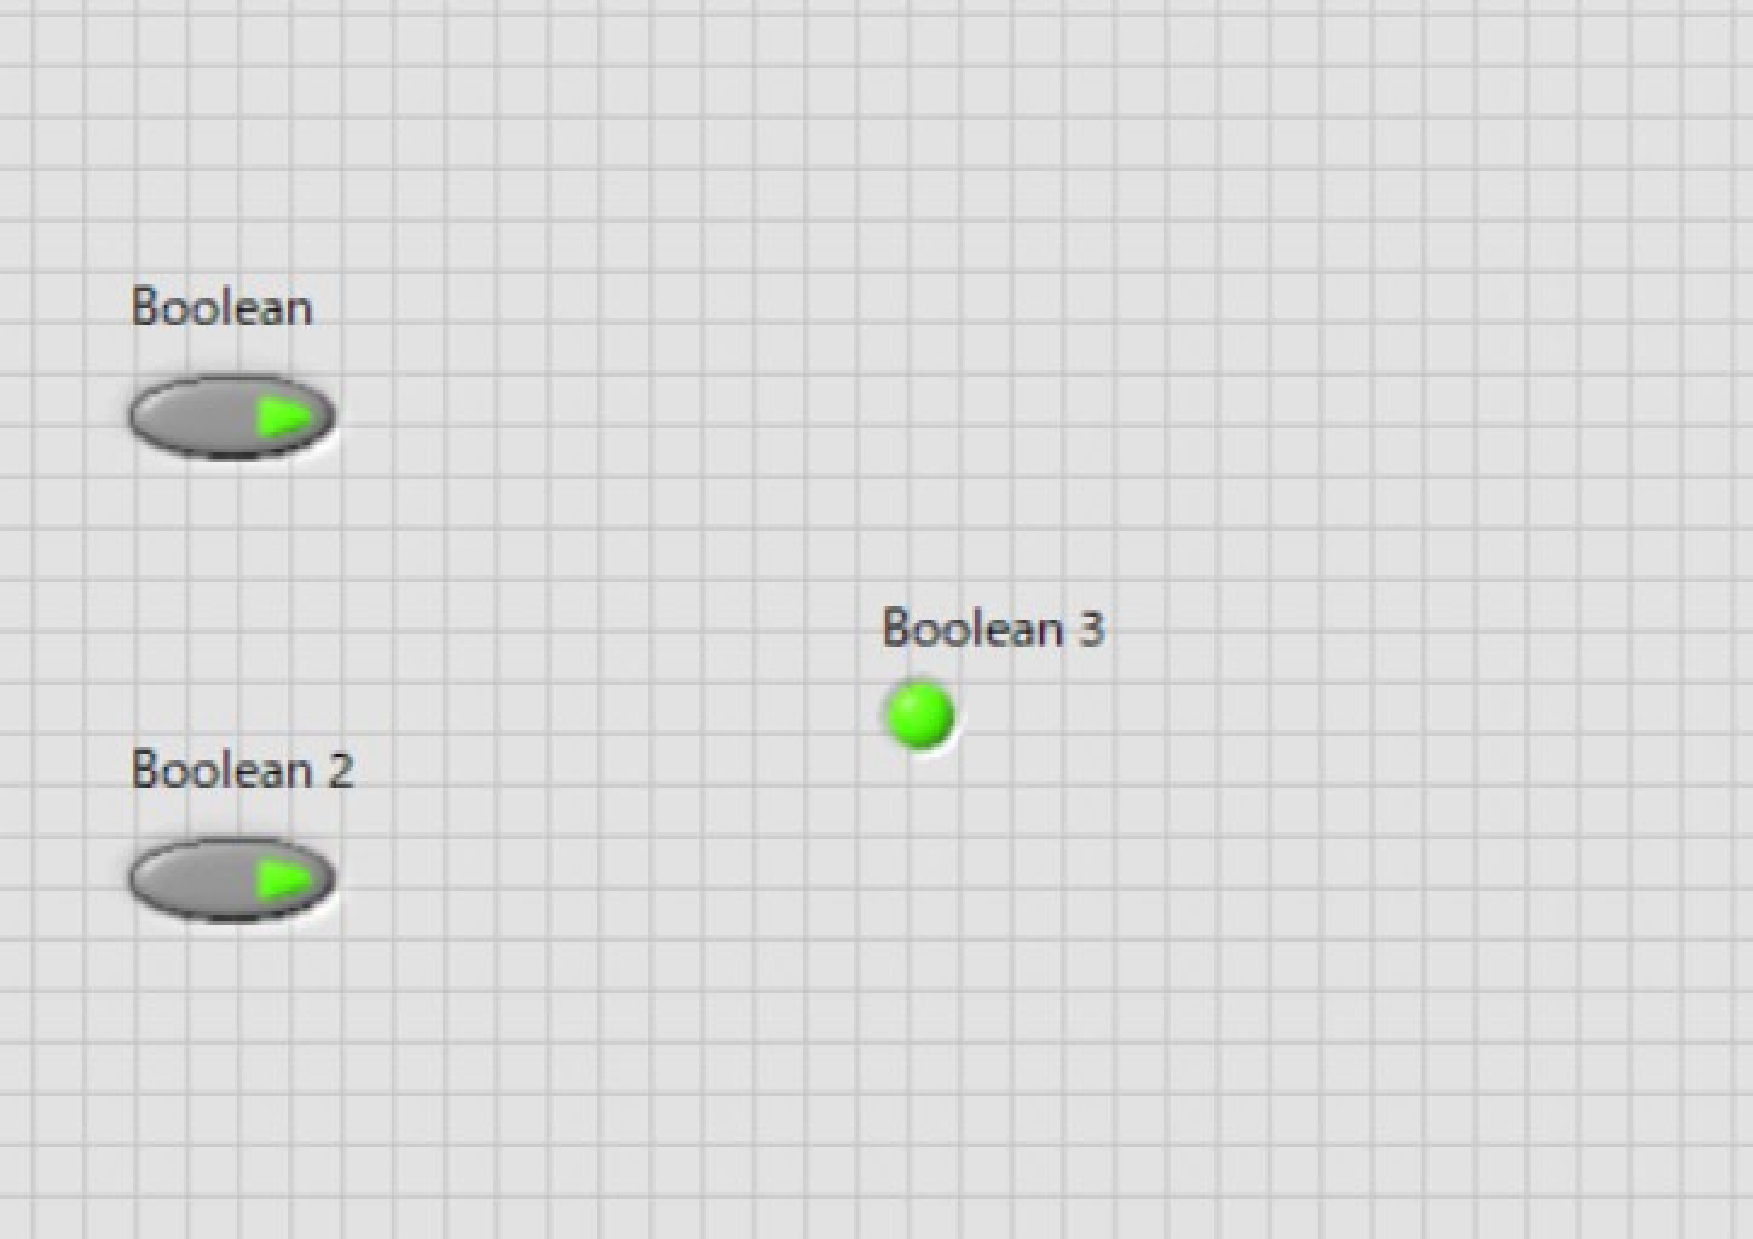
\includegraphics[width=100mm]{4-1f.pdf}
      \caption{(4)-(1) フロントパネル}
    \end{center}
  \end{figure}

  (4)-2について、ボタンを両方オフにしたときのみライトが消灯し、ほかの動作
  も試したが、ライトは点灯した。

  \begin{figure}[H]
    \begin{center}
      \includegraphics[width=100mm]{4-2f.pdf}
      \caption{(4)-(2) フロントパネル}
    \end{center}
  \end{figure}

  (4)-(3)について、ボタンを片方オンにしたときのみライトは点灯し、
  ほかの両方オン、両方オフも試したが、ライトは消灯した。

  \begin{figure}[H]
    \begin{center}
      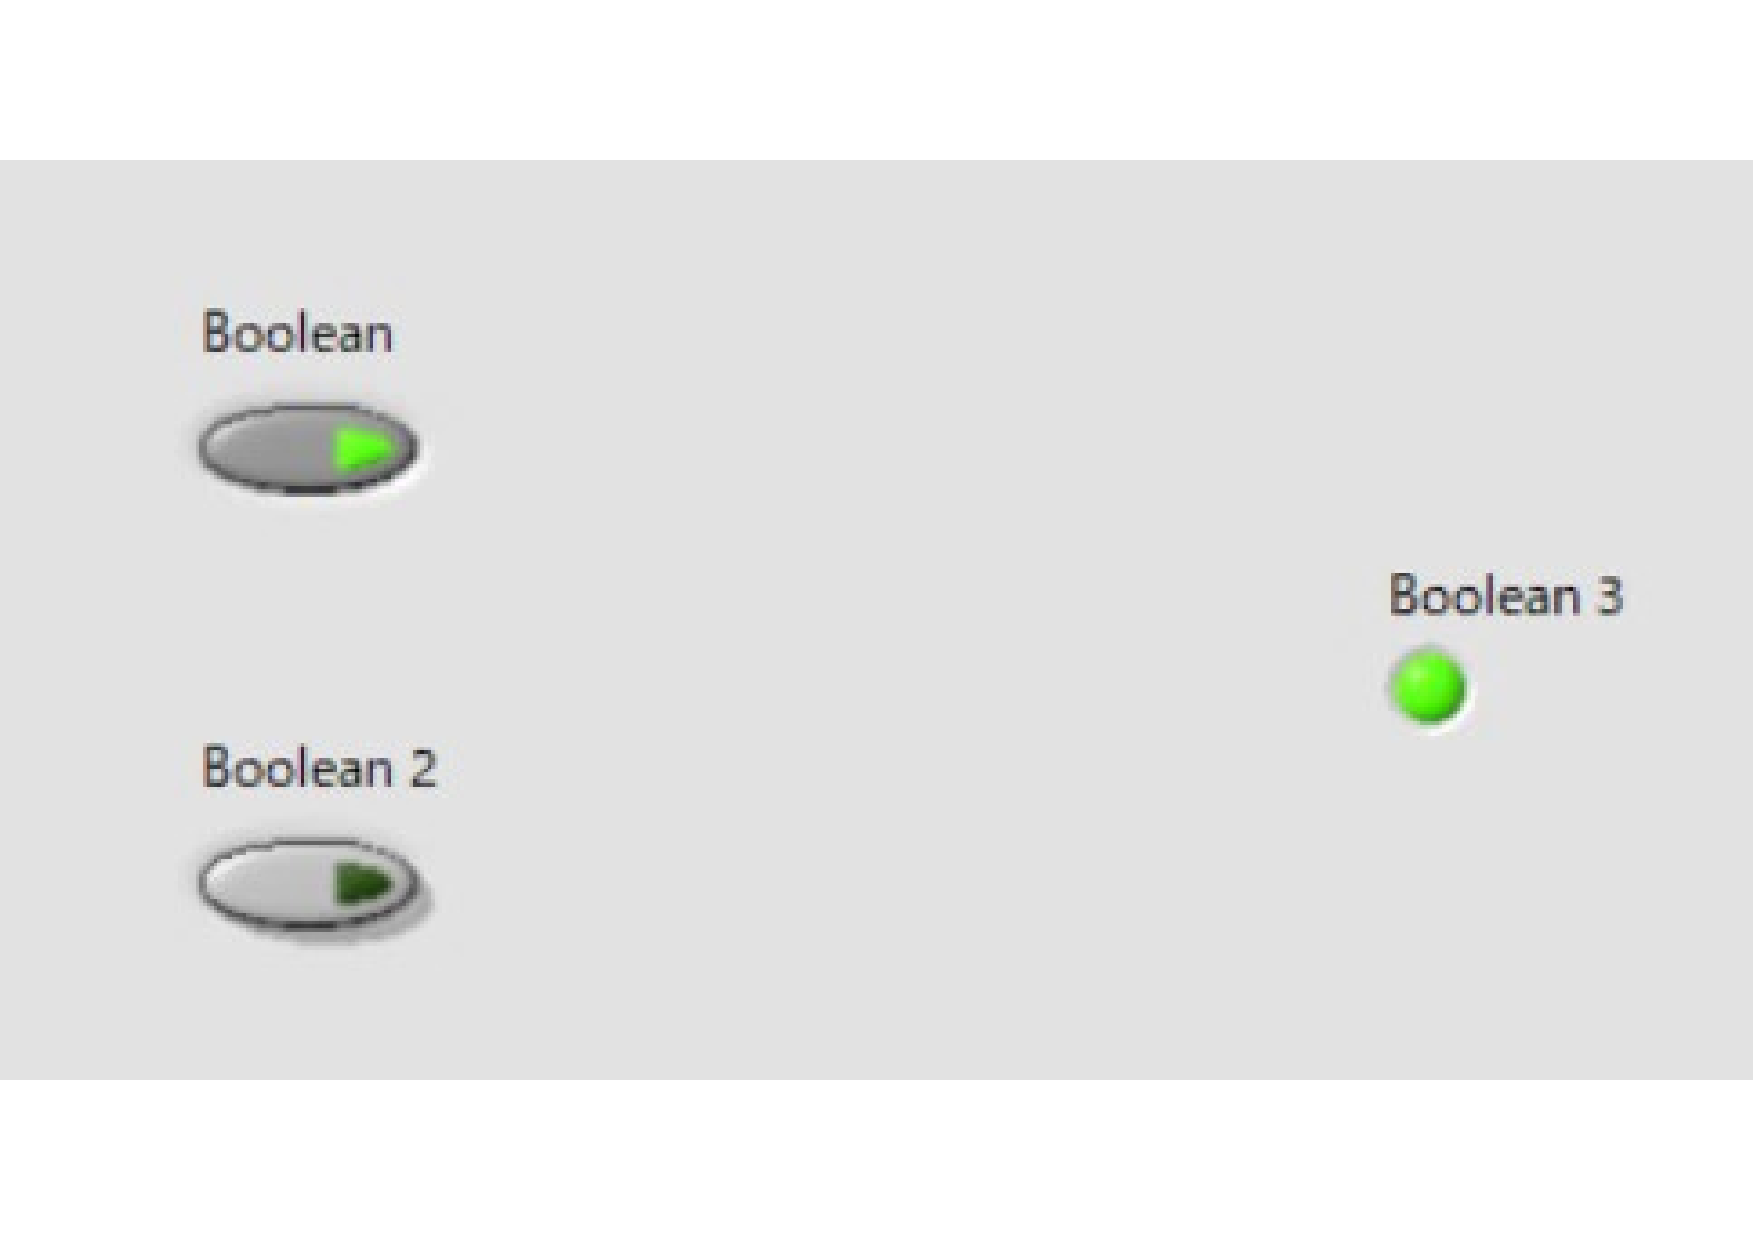
\includegraphics[width=100mm]{4-3f.pdf}
      \caption{(4)-(3) フロントパネル}
    \end{center}
  \end{figure}

電気回路練習問題の(1)においては、抵抗値としてそれぞれ3,4,4を、電圧として
それぞれ10,8を与えたところ、電流はそれぞれ1.2,0.4,1.6
この時、解行列

$X=\left(
  \begin{array}{r}
  1.2\\
  0.4
  \end{array}
\right)$、

抵抗行列は

$Y=\left(
  \begin{array}{rr}
  7 \ 4\\
  4 \ 8
  \end{array}
\right)$

を返した。

\begin{figure}[H]
  \begin{center}
    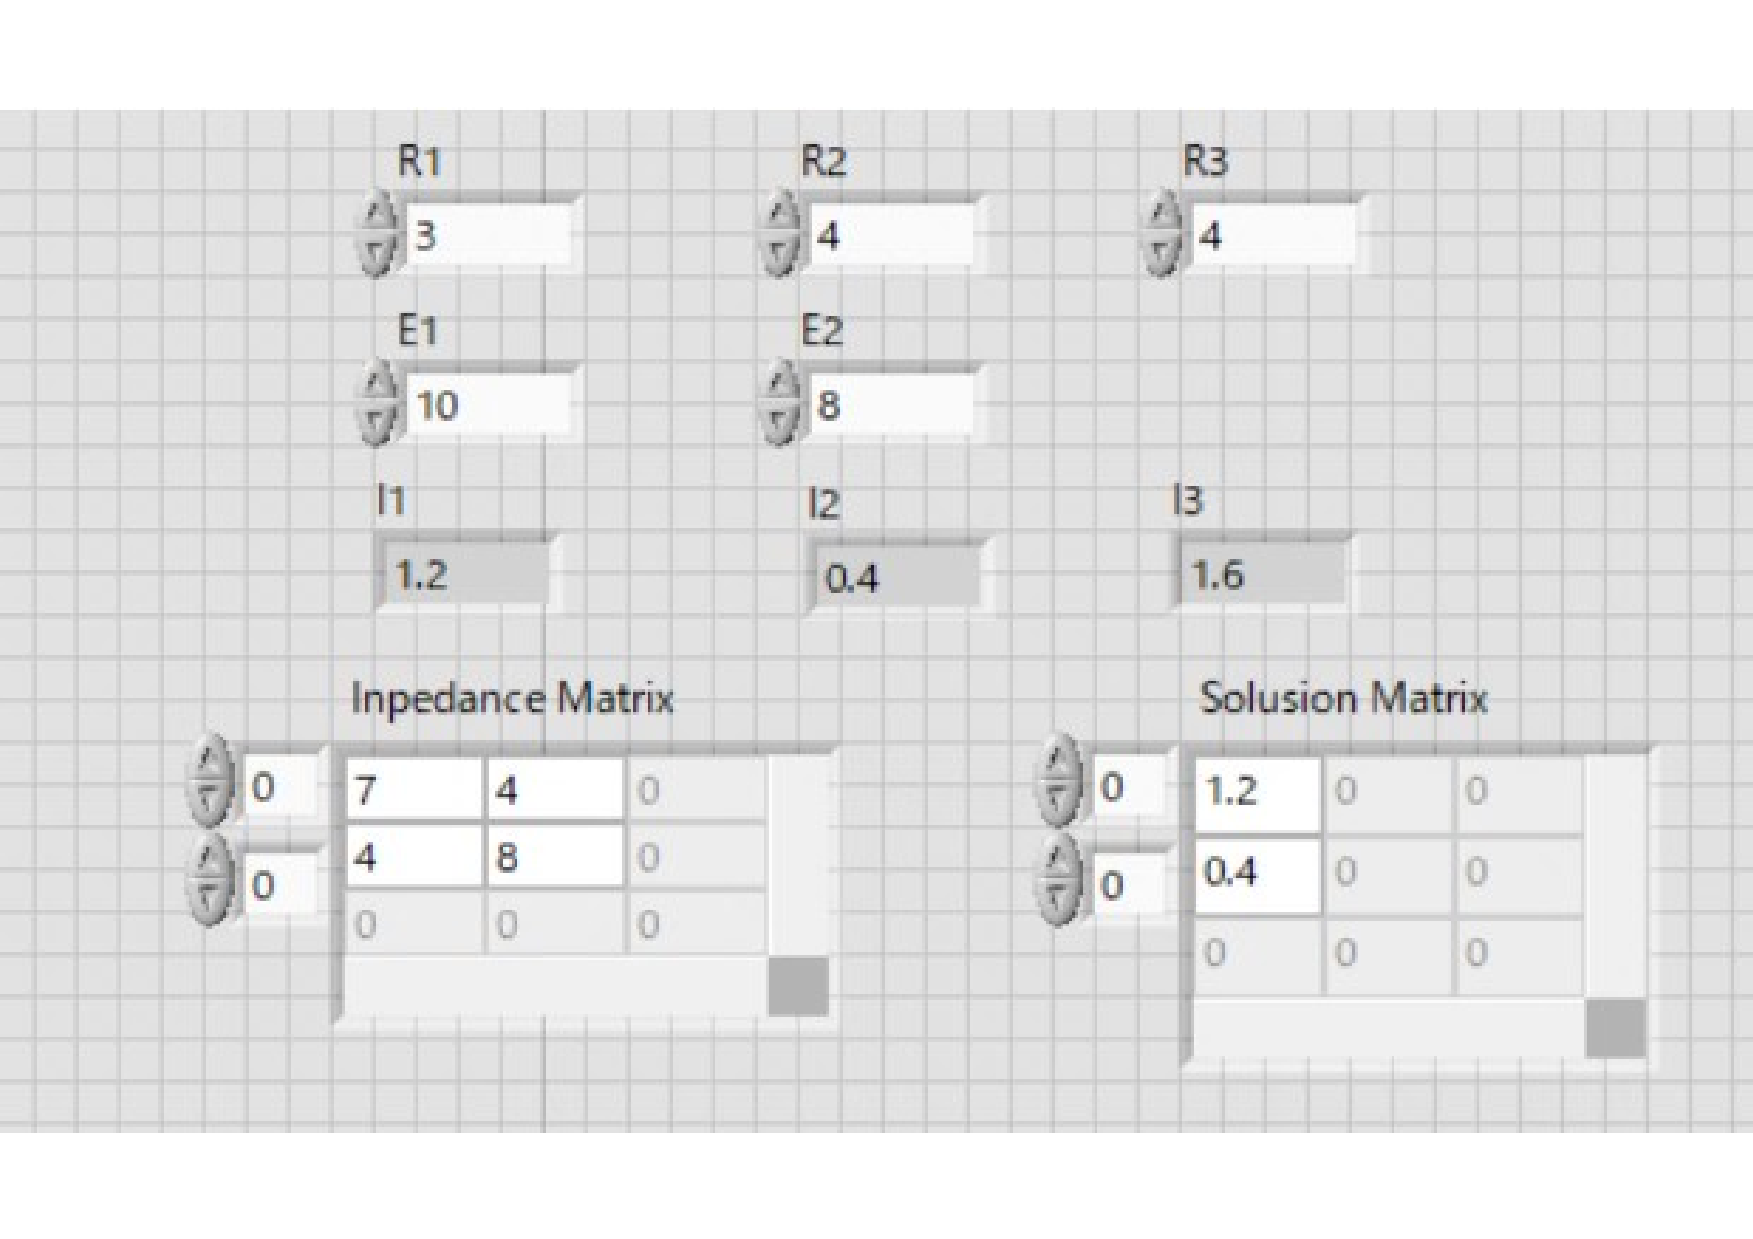
\includegraphics[width=100mm]{e3f.pdf}
    \caption{電気回路 フロントパネル}
  \end{center}
\end{figure}

判定処理練習問題の(3)については、私の身長体重である
161cm,56kgの値を入力してみたところ、
BMIは21.06、肥満度はNormal Rangeの値を返した。

\begin{figure}[H]
  \begin{center}
    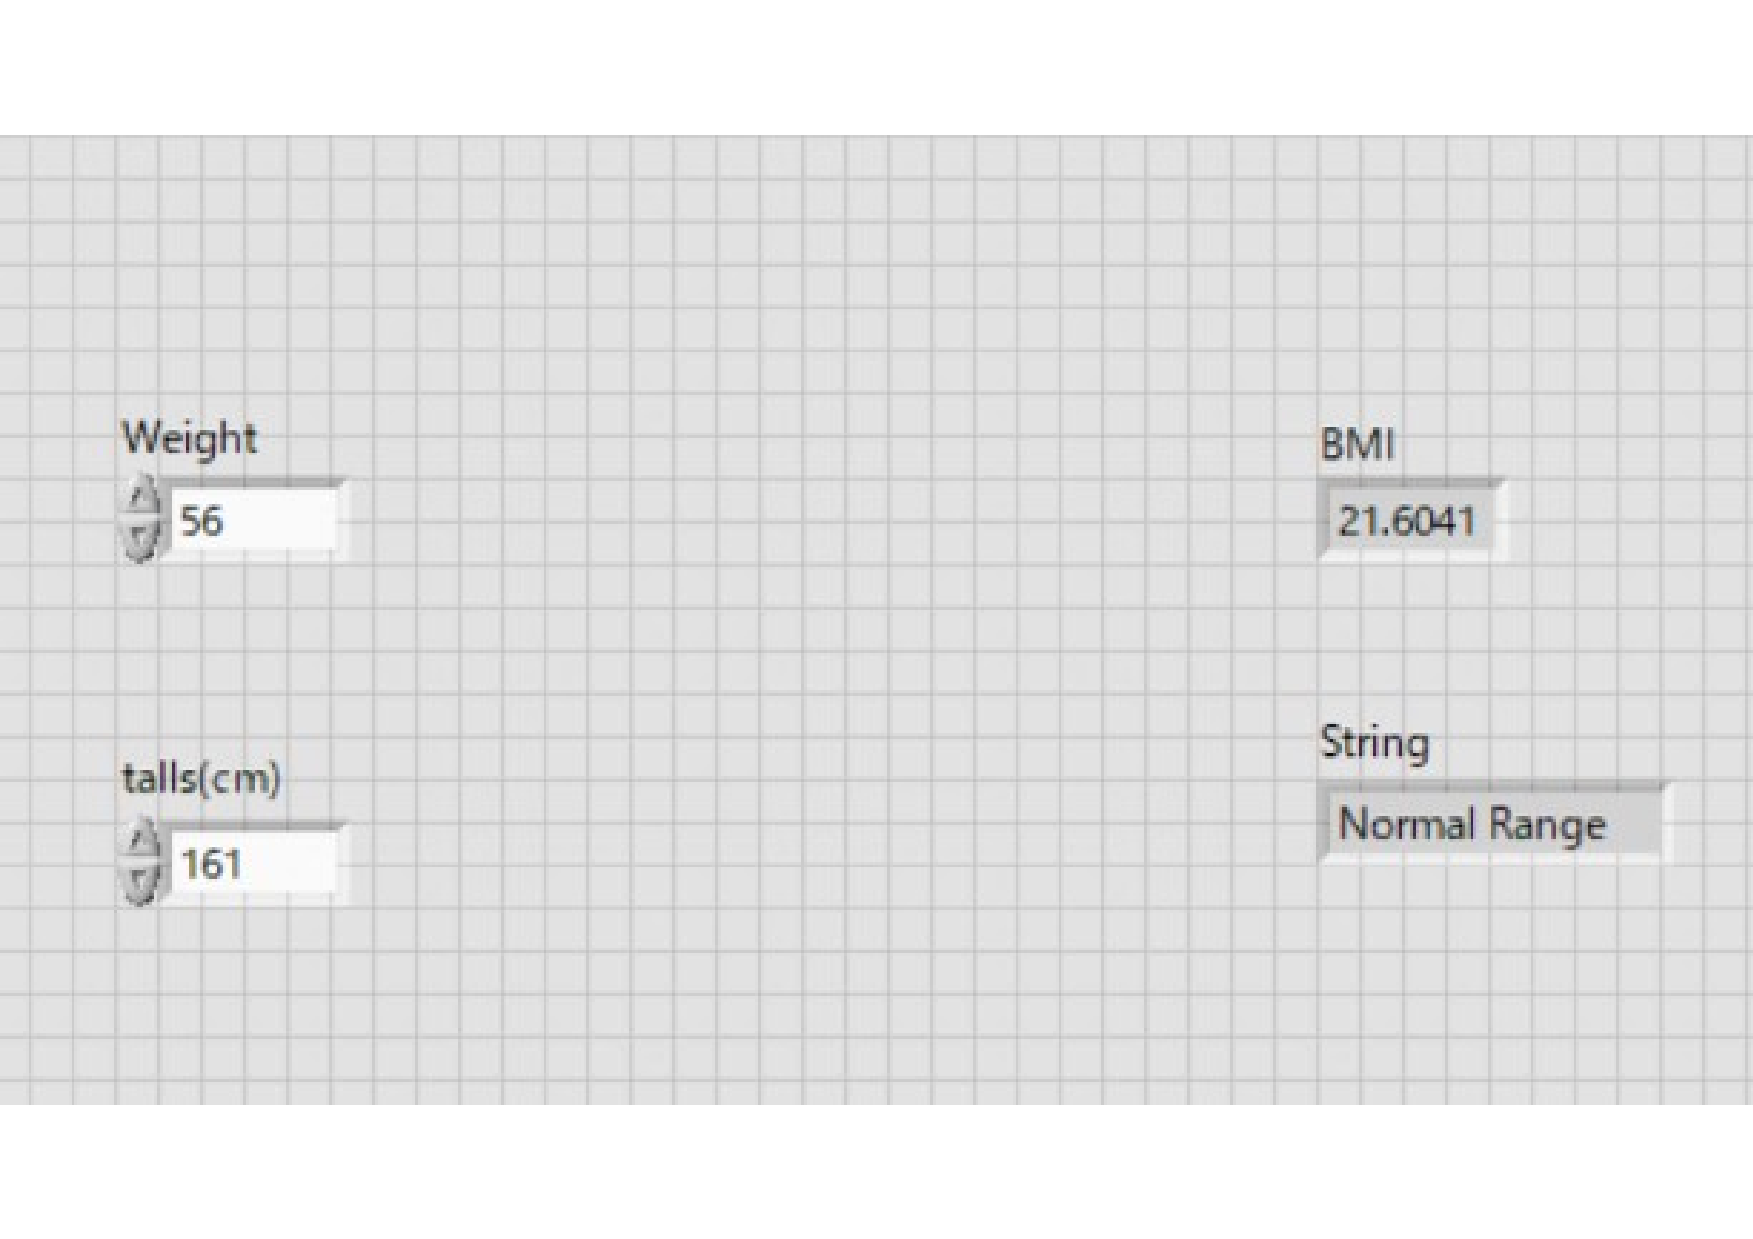
\includegraphics[width=100mm]{jadge3f.pdf}
    \caption{判定練習問題(1) フロントパネル}
  \end{center}
\end{figure}

  %%%%%%4章%%%%%%%%
  \section{考察}
  (4)は全般的にNANDで表現するといった問題だが、最初は何のことかさっぱりわからず、
  適当に試行錯誤していたが、TAから数学的な観点のアドバイスをもらい、数学的に
  NANDを表したうえでどうすればいいか、また各要素をNANDで表現する必要があるといった
  発想にいたることができたことが、NANDでの表現を成功させる工夫につながったと考えている。
  電気回路練習問題の(1)は模倣したので、特段の工夫はできていない。が、試行錯誤の
  段階では、四則演算を複雑に組み上げて直接求めようと考えていた。
  判定処理練習問題の(3)においては、case stractureではなくjadgeコンテクストを
  使用したこと、cm入力に対応させたことが工夫だが、jadgeコンテクストの発見が
  プログラムの整理につながり、エラーを防ぐことにつながったことは大きい。

  %%%%%%5章%%%%%%%%
  \section{感想}
  実験途中での発見もあるが、
  レポートの作成までを実験とするならば、
  実はこの授業での回路の理解は、このレポートをまとめている途中での発見もかなり
  多い。
  例えばorのNAND再現は実験途中はわからなかったことだが、
  まとめている時に数学的視点からの判定処理の理解が進み、各判定回路の再現を
  情報数学の知識を活用してできるようになり、情報数学の理解も進めることができた。
  また電気回路の問題では、途中にある様々なコンテクストの仕組みに気づき、
  なんとなく模倣して再現したlabviewでの行列の計算がなんと
  オウムの法則に則っているということを知り、線形代数学の活用によって効率的な
  計算ができるというに気づき、計算回路の仕組みまで理解できた。
  おそらく私が最初に知った線形代数学の物理への活用である。
  また、判定練習問題のjadgeも教えてもらって発見したことである。実験途中、
  case stractureで雑多な回路を組まなくていいと知ったときは感動を覚えた。
  これはついでなのだが、\LaTeX でこのレポートを書ききったことに対する喜びも
  またかなり大きい。
  %%%%%%6章%%%%%%%%
  \section{参考文献}
\begin{thebibliography}{9}
\bibitem{sankoga}
VI参考画像,
\begin{verbatim}
  https://kitaq-my.sharepoint.com/personal/hayami-t_kitakyu-u_ac_jp/_layouts/15/onedrive.aspx?id=%2Fpersonal%2Fhayami%2Dt%5Fkitakyu%2Du%5Fac%5Fjp%2FDocuments%2F%E3%82%B7%E3%82%B9%E3%83%86%E3%83%A0%E9%96%8B%E7%99%BA%E5%85%A5%E9%96%802022&ga=1
\end{verbatim}
\bibitem{siryou}
講義資料1,
\begin{verbatim}
  https://moodle.kitakyu-u.ac.jp/mod/resource/view.php?id=354156
\end{verbatim}
\end{thebibliography}
\end{document}